%!TEX program = xelatex
%%%%%%%%%%%%%%%%%%%%%%%%%%%%%%%%%%%%%%%%%%%
%\documentclass[12pt, a4paper, fullpage]{yzu_report}
%\documentclass[12pt, a4paper, fullpage]{uiucthesis}
\documentclass[12pt, a4paper, fullpage]{mythesis}

%\usepackage{definition}

%\usepackage{hyperref}

\usepackage{cite}
\usepackage{geometry}
\usepackage{amsmath}
\usepackage{amssymb}
\usepackage{mathrsfs}
\usepackage{listings}
\usepackage{amsthm} 

\newtheorem{definition}{Definition}[section]
\newtheorem{theorem}{Theorem}[section]
\newtheorem{lemma}{Lemma}[section]
%\newtheorem{proposition}{Proposition}

%\usepackage{ctex}
\usepackage{xmpmulti}
\usepackage{psfrag}
\usepackage{array}
\usepackage{graphicx}
\usepackage{caption}
\usepackage{subcaption}
\usepackage{booktabs}
\usepackage{threeparttable}
\usepackage{multirow}
\usepackage{footnote}
\usepackage{bm}
\usepackage{cases}
\usepackage{algorithm, algorithmic}
\usepackage{mathtools}
\usepackage{url}



\usepackage{color}
\usepackage{rotating}
\usepackage{multicol}
\usepackage{dcolumn}
\usepackage{indentfirst}
\usepackage{makecell}
\usepackage{leftidx}
\usepackage{slashbox}
%\usepackage{subfigure}
\usepackage{fancyhdr}
% 如果不需要任何浮水印,則請把下列介於 >>> 與 <<< 之間
% 的文字行關掉 (行首加上百分號)
%% 浮水印 >>> 
% !TEX root = Thesis.tex
% this file is encoded in utf-8
% v2.0 (Apr. 5, 2009)
% 如果浮水印不是全篇需要,請把下列介於 >>> 與 <<<
% 的「全篇浮水印專用碼」關掉 (行首加百分號)
% 參考自 Keith Reckdahl 寫的 "Using Imported Graphics in LATEX2e" (epslatex.pdf) p.39
% 如果只有特定頁需要浮水印
% 則依該頁屬性使用下列之一的命令 
% 普通頁命令 \thispagestyle{WaterMarkPage}
% plain 頁命令 \thispagestyle{PlainWaterMarkPage}
% empty 頁命令 \thispagestyle{EmptyWaterMarkPage}


% 將重複使用的浮水印章
% 圖檔是 my_watermark.xxx (nctu_logo)
% 副檔名可以不加,可以是 latex 系統能處裡的任何格式:pdf, gif, png, jpg, eps, ...
% 某些圖檔格式在某些工作流程可能需要作前置處裡。
% 例如,pdflatex 無法直接處理 eps 檔
%  latex + dvipdfmx 無法直接處理 pdf, gif, png, jpg, 需要用 ebb 小工具程式
%  對圖檔產生 .bb 對應檔。
%
% 寬為 5.1 cm
\newsavebox{\mywatermark}
\sbox{\mywatermark}{
\includegraphics[keepaspectratio,width=5.1cm]{nctu_logo}}


% 將 central header 擺放浮水印的巨集指令
\newcommand{\PlaceWaterMark}{\fancyhead[C]{\setlength{\unitlength}{1in}%
\begin{picture}(0,0)%
\put(-1,-6.2){\usebox{\mywatermark}}% 圖檔擺放的位置座標
\end{picture}}%
}

%\fancyhead{}  % reset left, central, right header to empty
%% 如果不需整篇論文都要浮水印
%% 則下面  >>> 與 <<< 之間的程式碼請關閉
%% >>> 全篇浮水印

\PlaceWaterMark  % 每一頁都有浮水印 (除了 plain、empty 頁以外)

% 重新定義 plain 頁面
% 每張 plain 頁面 (每一章的第一頁) 也加浮水印

%\fancypagestyle{plain}{%
%\fancyhead{}%
%\PlaceWaterMark%
%\fancyfoot{}%
%\fancyfoot[C]{\thepage}
%\renewcommand{\headrulewidth}{0pt}%
%\renewcommand{\footrulewidth}{0pt}%
%}
%% <<< 全篇浮水印

%% 如果只有一、兩頁需要有浮水印
%% 可以在該頁 (有頁碼) 使用 \thispagestyle{WaterMarkPage}
%% 此命令不影響原有的 header、footer
%\fancypagestyle{WaterMarkPage}{%
%\PlaceWaterMark%
%}

%% 如果只有一、兩頁 plain 頁需要有浮水印 (如 摘要、自傳等)
%% 可以在該頁 (有頁碼) 使用 \thispagestyle{PlainWaterMarkPage}
%% 只有頁碼與浮水印,沒有其他的 header、footer
%% 等同於 plain page style + water mark
%\fancypagestyle{PlainWaterMarkPage}{%
%\fancyhead{}%
%\PlaceWaterMark%
%\fancyfoot{}%
%\fancyfoot[C]{\thepage}
%\renewcommand{\headrulewidth}{0pt}%
%\renewcommand{\footrulewidth}{0pt}%
%}

%% 如果只有一、兩頁 empty 頁需要有浮水印 (如封面、書名頁)
%% 可以在該頁 (無頁碼) 使用 \thispagestyle{EmptyWaterMarkPage}
%% 等同於 empty page style + water mark
\fancypagestyle{EmptyWaterMarkPage}{%
\fancyhead{}%
%\PlaceWaterMark%
\fancyfoot{}%
\renewcommand{\headrulewidth}{0pt}%
\renewcommand{\footrulewidth}{0pt}%
}
%% <<< 浮水印


\pagenumbering{arabic}

\usepackage{geometry}  % for easy margin settings
% margins setting
%\geometry{verbose,a4paper,tmargin=2.5cm,bmargin=3.5cm,lmargin=2.5cm,rmargin=2cm}



\geometry{verbose,a4paper,tmargin=2.5cm,bmargin=3.5cm,lmargin=2.5cm,rmargin=2.5cm}

\makesavenoteenv{tabular}
\renewcommand{\labelenumi}{\alph{enumi})}
%\theoremstyle{remark}
\newtheoremstyle{mythmsty}{3pt}{3pt}{}{}{\bf}{.}{.5em}{}
\theoremstyle{mythmsty}
\newtheorem{proposition}{Proposition}[chapter]
%% ENVIRONEMTS
\def\QED{\mbox{\rule[0pt]{1.5ex}{1.5ex}}}
\def\myproof{\noindent\hspace{2em}{\it Proof: }}
\def\endmyproof{\hspace*{\fill}~\QED\par\endtrivlist\unskip}
%%%%%%%%%%%%%%%%%%%%%%%%%%%%%%%%

\usepackage{type1cm}
\usepackage{fontspec}			        %加這個就可以設定字體
\usepackage{xeCJK} 			            %讓中英文字體分開設置
\XeTeXlinebreaklocale "zh"           	%這兩行一定要加,中文才能自動換行
\XeTeXlinebreakskip = 0pt plus 1pt   	%這兩行一定要加,中文才能自動換行
			                        				%加了這幾行後,就可以隨意的打中文,接下來的跟一般的LaTeX都一樣
			                        				%注意!!!一定要存成UTF-8編碼的文件。

%\setCJKmainfont[AutoFakeBold=6,AutoFakeSlant=.4]{標楷體}
								%設定中文為系統上的字型,而英文不去更動,使用原TeX字型
               	%AutoFakeBold設定粗體字要多粗
                %AutoFakeSlant設定斜體字要多斜,範圍-0.999到0.999,負值為往左斜
%\defaultCJKfontfeatures{AutoFakeBold=6,AutoFakeSlant=.4} %以後不用再設定粗斜
\setCJKmainfont[AutoFakeBold=6,AutoFakeSlant=.4]{[BiauKai.ttf]}
\defaultCJKfontfeatures{AutoFakeBold=6,AutoFakeSlant=.4}
\newCJKfontfamily\Kai{[BiauKai.ttf]}       	%定義指令\Kai則切換成標楷體
%\newCJKfontfamily\Hei{微軟正黑體}   	%定義指令\Hei則切換成正黑體
%\newCJKfontfamily\NewMing{新細明體} 	%定義指令\NewMing則切換成新細明體


%%%%%%%%%%%%%%%%%%%%%%%%%%%%%%%%
\begin{document}

%\title{Parallel Turbo Decoder Design and Implementation}  
%\author{Cheng-Chi Wong}
%\phdthesis
%\department{Department of Electronics Engineering \& Institute of Electronics}
%\college{Electrical \& Computer Engineering} 
%\advisor{Hsie-Chia Chang}
%\degreeyear{2010}

%\maketitle

\frontmatter

% !TEX root = Thesis.tex
%
% this file is encoded in utf-8
% v2.0 (Apr. 5, 2009)

% ??????????????????????
% ??????????? (??) ??
% ?? \prechaptername ???? Chapter
% ?? \postchaptername ???????
% ?? \tablename ???? Table
% ?? \figurename ???? Figure
%\renewcommand\prechaptername{?} % ???????????? x ??
%\renewcommand\postchaptername{?}
%\renewcommand{\tablename}{?} % ???? table caption ???? x???
%\renewcommand{\figurename}{?} % ???? figure caption ???? x???

% ??????????????????????? (??????????)
%\newcommand{\nameInnerCover}{???}
%\newcommand{\nameCommitteeForm}{?????????}
%\newcommand{\nameCopyrightForm}{???}
%\newcommand{\nameCabstract}{????}
%\newcommand{\nameEabstract}{????}
%\newcommand{\nameAckn}{??}
%\newcommand{\nameToc}{??}
%\newcommand{\nameLot}{???}
%\newcommand{\nameTof}{???}
%\newcommand{\nameSlist}%{????}
\newcommand{\nameSlist}{Symbol List}
%\newcommand{\nameRef}{????}
%\newcommand{\nameVita}{??}


%!TEX root = Thesis.tex
%
% this file is encoded in utf-8
% v2.0 (Apr. 5, 2009)
% do not change the content of this file
% unless the thesis layout rule is changed
% 無須修改本檔內容,除非校方修改了
% 封面、書名頁、中文摘要、英文摘要、誌謝、目錄、表目錄、圖目錄、符號說明
% 等頁之格式


% default variables definitions
% 此處只是預設值,不需更改此處
% 請更改 my_names.tex 內容
\newcommand\cTitle{論文題目}
\newcommand\eTitle{MY THESIS TITLE}
\newcommand\myCname{我的中文名字}
\newcommand\myEname{My Name}
\newcommand\advisorCnameA{第一指導教授中文名字}
\newcommand\advisorEnameA{Name of the 1st Advisor}
\newcommand\advisorCnameB{第二指導教授中文名字}
\newcommand\advisorEnameB{Name of the 2nd Advisor}
\newcommand\advisorCnameC{第三指導教授中文名字}
\newcommand\advisorEnameC{Name of the 3rd Advisor}
\newcommand\univCname{大學名稱}
\newcommand\univEname{University}
\newcommand\deptCname{系所名稱}
\newcommand\fulldeptEname{Department}
\newcommand\deptEname{Department}
\newcommand\collEname{College}
\newcommand\degreeCname{學位}
\newcommand\degreeEname{Degree}
\newcommand\cYear{民國年份}
\newcommand\cMonth{月數}
\newcommand\eYear{Year}
\newcommand\eMonth{Month}
\newcommand\ePlace{Location of University}

% user's names; to replace those default variable definitions
% this file is encoded in utf-8
% v2.0 (Apr. 5, 2009)
% 填入你的論文題目、姓名等資料
% 如果題目內有必須以數學模式表示的符號,請用 \mbox{} 包住數學模式,如下範例
% 如果中文名字是單名,與姓氏之間建議以全形空白填入,如下範例
% 英文名字中的稱謂,如 Prof. 以及 Dr.,其句點之後請以不斷行空白~代替一般空白,如下範例
% 如果你的指導教授沒有如預設的三位這麼多,則請把相對應的多餘教授的中文、英文名
%    的定義以空的大括號表示
%    如,\renewcommand\advisorCnameB{}
%          \renewcommand\advisorEnameB{}
%          \renewcommand\advisorCnameC{}
%          \renewcommand\advisorEnameC{}

% 論文題目 (中文)
\renewcommand\cTitle{類比電路自動化與遷移設計之研究}

% 論文題目 (英文)
\renewcommand\eTitle{Research on Analog Design Automation and Migration}

% 我的姓名 (中文)
\renewcommand\myCname{潘柏丞}

% 我的姓名 (英文)
\renewcommand\myEname{Po-Cheng Pan}

% 指導教授A的姓名 (中文)
\renewcommand\advisorCnameA{陳宏明}

% 指導教授A的姓名 (英文)
\renewcommand\advisorEnameA{Hung-Ming Chen}

% 指導教授B的姓名 (中文)
\renewcommand\advisorCnameB{}

% 指導教授B的姓名 (英文)
\renewcommand\advisorEnameB{}

% 指導教授C的姓名 (中文)
\renewcommand\advisorCnameC{}

% 指導教授C的姓名 (英文)
\renewcommand\advisorEnameC{}

% 校名 (中文)
\renewcommand\univCname{國立交通大學}

% 校名 (英文)
\renewcommand\univEname{National Chiao Tung University}

% 系所名 (中文)
\renewcommand\deptCname{電子工程學系電子研究所}

% 系所全名 (英文)
\renewcommand\fulldeptEname{Department of Electronics Engineering \& Institute of Electronics}

% 系所短名 (英文, 用於書名頁學位名領域)
\renewcommand\deptEname{Electronics Engineering}

% 學院英文名 (如無,則以空的大括號表示)
\renewcommand\collEname{College of Electrical and Computer Engineering}

% 學位名 (中文)
\renewcommand\degreeCname{博士}

% 學位名 (英文)
\renewcommand\degreeEname{Doctor of Philosophy}

% 口試年份 (中文、民國)
\renewcommand\cYear{一零四}

% 口試月份 (中文)
\renewcommand\cMonth{五} 

% 口試年份 (阿拉伯數字、西元)
\renewcommand\eYear{2015} 

% 口試月份 (英文)
\renewcommand\eMonth{May}

% 學校所在地 (英文)
\renewcommand\ePlace{Hsinchu, Taiwan, Republic of China}

%畢業級別;用於書背列印;若無此需要可忽略
\newcommand\GraduationClass{103}

%%%%%%%%%%%%%%%%%%%%%%


% make the line spacing in effect
%\newcommand{\mybaselinestretch}{1.5}  %行距 1.5 倍 + 20%, (約為 double space)
%\renewcommand{\baselinestretch}{\mybaselinestretch}  % 論文行距預設值
%\parskip = 2ex                                       % 段落之間的間隔為兩個 x 的高度
%\parindent = 0Pt                                     % 這裡設成不內縮

%\renewcommand{\baselinestretch}{\mybaselinestretch}
\large % it needs a font size changing command to be effective

\newcommand\itsempty{}
%%%%%%%%%%%%%%%%%%%%%%%%%%%%%%%
%        cover 封面
%%%%%%%%%%%%%%%%%%%%%%%%%%%%%%%

\begin{titlepage}
% no page number
% next page will be page 1

\ifx\mywatermark\undefined 
  \thispagestyle{empty}  % 無頁碼、無 header (無浮水印)
\else
  \thispagestyle{EmptyWaterMarkPage} % 無頁碼、有浮水印
\fi

% aligned to the center of the page
\begin{center}
% font size (relative to 12 pt):
% \large (14pt) < \Large (18pt) < \LARGE (20pt) < \huge (24pt)< \Huge (24 pt)
%
%\makebox[12cm][s]{\Huge{\univCname}}\\  %顯示中文校名
\makebox[12cm][s]{\fontsize{36pt}{10pt}\selectfont{\univCname}}\\
\vspace{1.5cm}
%\makebox[12cm][s]{\huge{\deptCname}}\\ %顯示中文系所名
\makebox[12cm][s]{\fontsize{28pt}{10pt}\selectfont{\deptCname}}\\
\vspace{1.5cm}
%\makebox[6cm][s]{\huge{\degreeCname 論文}}\\ %顯示論文種類 (中文)
\makebox[6cm][s]{\fontsize{28pt}{10pt}\selectfont{\degreeCname 論文}}\\
\vspace{2cm}
%
% Set the line spacing to single for the titles (to compress the lines)
%\renewcommand{\baselinestretch}{1}   %行距 1 倍
\large % it needs a font size changing command to be effective
\LARGE{\cTitle}\\  % 中文題目
%
%\vspace{1cm}
%
\LARGE{\eTitle}\\ %英文題目
\vspace{2cm}
% \makebox is a text box with specified width;
% option s: stretch
% use \makebox to make sure
% 「研究生:」 與「指導教授:」occupy the same width
\hspace{4.5cm} \makebox[4cm][s]{\LARGE{研究生}} \makebox[0.5cm][c]{\LARGE{:}}
\LARGE{\myCname}  % 顯示作者中文名
\hfill \makebox[1cm][s]{}\\
%
\hspace{4.5cm} \makebox[4cm][s]{\LARGE{指導教授}}  \makebox[0.5cm][c]{\LARGE{:}}
\LARGE{\advisorCnameA}  %顯示指導教授A中文名
\hfill \makebox[1cm][s]{}\\
%
% 判斷是否有共同指導的教授 B
\ifx \advisorCnameB  \itsempty
\relax % 沒有 B 教授,所以不佔版面,不印任何空白
\else
% 共同指導的教授 B
\hspace{4.5cm} \makebox[4cm][s]{} \makebox[0.5cm][c]{}
\LARGE{\advisorCnameB}  %顯示指導教授B中文名
\hfill \makebox[1cm][s]{}\\
\fi
%
% 判斷是否有共同指導的教授 C
\ifx \advisorCnameC  \itsempty
\relax % 沒有 C 教授,所以不佔版面,不印任何空白
\else
% 共同指導的教授 C
\hspace{4.5cm} \makebox[3cm][s]{}
\LARGE{\advisorCnameC}  %顯示指導教授C中文名
\hfill \makebox[1cm][s]{}\\
\fi
%
\vfill
\makebox[10cm][s]{\LARGE{中華民國\cYear 年\cMonth 月}}%
%
\end{center}
% Resume the line spacing to the desired setting
%\renewcommand{\baselinestretch}{\mybaselinestretch}   %恢復原設定
% it needs a font size changing command to be effective
% restore the font size to normal
\normalsize
\end{titlepage}
%%%%%%%%%%%%%%

%% 從摘要到本文之前的部份以小寫羅馬數字印頁碼
% 但是從「書名頁」(但不印頁碼) 就開始計算
\setcounter{page}{1}
\pagenumbering{roman}
%%%%%%%%%%%%%%%%%%%%%%%%%%%%%%%
%       書名頁 
%%%%%%%%%%%%%%%%%%%%%%%%%%%%%%%
\newpage

% 判斷是否要浮水印?
\ifx\mywatermark\undefined 
  \thispagestyle{empty}  % 無頁碼、無 header (無浮水印)
\else
  \thispagestyle{EmptyWaterMarkPage} % 無頁碼、有浮水印
\fi

%no page number
% create an entry in table of contents for 書名頁
%%\phantomsection % for hyperref to register this
%%\addcontentsline{toc}{chapter}{\nameInnerCover}


% aligned to the center of the page
\begin{center}
% font size (relative to 12 pt):
% \large (14pt) < \Large (18pt) < \LARGE (20pt) < \huge (24pt)< \Huge (24 pt)
% Set the line spacing to single for the titles (to compress the lines)
%%\renewcommand{\baselinestretch}{1}   %行距 1 倍
% it needs a font size changing command to be effective
%中文題目
\Large{\cTitle}\\ %%%%%
%\vspace{1cm}
% 英文題目
\Large{\eTitle}\\ %%%%%
%\vspace{1cm}
\vfill
% \makebox is a text box with specified width;
% option s: stretch
% use \makebox to make sure
% 「研究生:」 與「指導教授:」occupy the same width
\makebox[3cm][s]{\large{研 究 生}} \makebox{\large{:}}
\makebox[3cm][l]{\large{\myCname}} %%%%%
\hfill
\makebox[1.5cm][s]{\large{Student}} \makebox{\large{:}}
\makebox[5cm][l]{\large{\myEname}}\\ %%%%%
%
%\vspace{1cm}
%
\makebox[3cm][s]{\large{指導教授}} \makebox{\large{:}}
\makebox[4cm][l]{\large{\advisorCnameA} \large{博士}} %%%%%
%\makebox[1cm][l]{\large{博士}}
\hfill
\makebox[1.5cm][s]{\large{Advisor}} \makebox{\large{:}}
\makebox[5cm][l]{\large{Dr. \advisorEnameA}}\\ %%%%%
%
% 判斷是否有共同指導的教授 B
\ifx \advisorCnameB  \itsempty
\relax % 沒有 B 教授,所以不佔版面,不印任何空白
\else
%共同指導的教授B
\makebox[3cm][s]{}
%\makebox[3cm][l]{\large{\advisorCnameB}} %%%%%
\makebox[0.5cm][l]{}
\makebox[4cm][l]{\large{\advisorCnameB} \large{博士}} %%%%%
\hfill
\makebox[2cm][s]{}
\makebox[5cm][l]{\large{Dr. \advisorEnameB}}\\ %%%%%%%%%%%%%%%%%%%%%%%%%%%%%%%%%%%%%%%%%%%%%%%%%%%%%%%%%%%%%%%%%%%%%%%%%%%%%%%%%%%%%%%%%%%%%%%%%%%%%%%%%%%%%%%%%%%%%
\fi
%
% 判斷是否有共同指導的教授 C
\ifx \advisorCnameC  \itsempty
\relax % 沒有 C 教授,所以不佔版面,不印任何空白
\else
%共同指導的教授C
\makebox[3cm][s]{}
\makebox[3cm][l]{\large{\advisorCnameC}} %%%%%
\hfill
\makebox[2cm][s]{}
\makebox[5cm][l]{\large{\advisorEnameC}}\\ %%%%%
\fi
%
% Resume the line spacing to the desired setting
%\renewcommand{\baselinestretch}{\mybaselinestretch}   %恢復原設定
\large %it needs a font size changing command to be effective
%
\vfill
\makebox[4cm][s]{\large{\univCname}}\\% 校名
\makebox[6cm][s]{\large{\deptCname}}\\% 系所名
\makebox[3cm][s]{\large{\degreeCname 論文}}\\% 學位名
%
%\vspace{1cm}
\vfill
%%\large{A Dissertation}\\%
\normalsize{A Dissertation}\\
%%\large{Submitted to}%
\normalsize{Submitted to}
%
%%\large{\fulldeptEname}\\%系所全名 (英文)
\normalsize{\fulldeptEname}\\
%
%
\ifx \collEname  \itsempty
\relax % 沒有學院名 (英文),所以不佔版面,不印任何空白
\else
% 有學院名 (英文)
%%\large{\collEname}\\% 學院名 (英文)
\normalsize{\collEname}\\
\fi
%
%%\large{\univEname}\\%校名 (英文)
\normalsize{\univEname}\\
%
%%\large{in Partial Fulfillment of the Requirements}\\
\normalsize{in Partial Fulfillment of the Requirements}\\
%
%%\large{for the Degree of}
\normalsize{for the Degree of}
%
%%\large{\degreeEname}\\%學位名(英文)
\normalsize{\degreeEname}\\
%
%%\large{in}\\
\normalsize{in}\\
%
%%\large{\deptEname}\\%系所短名(英文;表明學位領域)
\normalsize{\deptEname}\\
%
%%\large{\eMonth\ \eYear}\\%月、年 (英文)
\normalsize{\eMonth\ \eYear}\\
%
%%\large{\ePlace}% 學校所在地 (英文)
\normalsize{\ePlace}% 學校所在地 (英文)
\vfill
\large{中華民國}%
\large{\cYear}% %%%%%
\large{年}%
\large{\cMonth}% %%%%%
\large{月}\\
\end{center}
% restore the font size to normal
\normalsize
\clearpage


%%%%%%%%%%%%%%%%%%%%%%%%%%%%%%%
%       論文口試委員審定書 (計頁碼,但不印頁碼) 
%%%%%%%%%%%%%%%%%%%%%%%%%%%%%%%


%%%%%%%%%%%%%%%%%%%%%%%%%%%%%%%
%       授權書 (計頁碼,但不印頁碼) 
%%%%%%%%%%%%%%%%%%%%%%%%%%%%%%%

























%%%%%%%%%%%%%%%%%%%%%%%%%%%%%%%%
%%       中文摘要 
%%%%%%%%%%%%%%%%%%%%%%%%%%%%%%%%
%
\newpage
\thispagestyle{plain}  % 無 header,但在浮水印模式下會有浮水印

% create an entry in table of contents for 中文摘要
%%\phantomsection % for hyperref to register this
%%\addcontentsline{toc}{chapter}{\nameCabstract}

% aligned to the center of the page
\begin{center}
% font size (relative to 12 pt):
% \large (14pt) < \Large (18pt) < \LARGE (20pt) < \huge (24pt)< \Huge (24 pt)
% Set the line spacing to single for the names (to compress the lines)
%%\renewcommand{\baselinestretch}{1}   %行距 1 倍
% it needs a font size changing command to be effective
\Large{\cTitle}\\  %中文題目
\vspace{0.83cm}
% \makebox is a text box with specified width;
% option s: stretch
% use \makebox to make sure
% each text field occupies the same width
\makebox[1.5cm][s]{\large{學生:}}
\makebox[3cm][l]{\large{\myCname}} %學生中文姓名
\hfill
%
\makebox[3cm][s]{\large{指導教授:}}
\makebox[3cm][l]{\large{\advisorCnameA}\large{教授}} \\ %教授A中文姓名
%
% 判斷是否有共同指導的教授 B
\ifx \advisorCnameB  \itsempty
\relax % 沒有 B 教授,所以不佔版面,不印任何空白
\else
%共同指導的教授B
\makebox[1.5cm][s]{}
\makebox[3cm][l]{} %%%%%
\hfill
\makebox[3cm][s]{}
\makebox[3cm][l]{\large{\advisorCnameB}\large{教授}}\\ %教授B中文姓名
\fi
%
% 判斷是否有共同指導的教授 C
\ifx \advisorCnameC  \itsempty
\relax % 沒有 C 教授,所以不佔版面,不印任何空白
\else
%共同指導的教授C
\makebox[1.5cm][s]{}
\makebox[3cm][l]{} %%%%%
\hfill
\makebox[3cm][s]{}
\makebox[3cm][l]{\large{\advisorCnameC}\large{教授}}\\ %教授C中文姓名
\fi
%
\vspace{0.42cm}
%
\large{\univCname}\large{\deptCname}\\ %校名系所名
\vspace{0.83cm}
%\vfill
\makebox[2.5cm][s]{\large{摘要}}\\
\end{center}
% Resume the line spacing to the desired setting
%%\renewcommand{\baselinestretch}{\mybaselinestretch}   %恢復原設定
%it needs a font size changing command to be effective
% restore the font size to normal
\normalsize
%%%%%%%%%%%%%
% !TEX root = Thesis.tex

在積體電路的範疇,為了更有效地達到先進製程底下的電路效能,類比電路的自動化已不容忽視。以下自行發揮

























%%%%%%%%%%%%%%%%%%%%%%%%%%%%%%%
%       英文摘要 
%%%%%%%%%%%%%%%%%%%%%%%%%%%%%%%
%
\newpage
\thispagestyle{plain}  % 無 header,但在浮水印模式下會有浮水印

% create an entry in table of contents for 英文摘要
%%\phantomsection % for hyperref to register this
%%\addcontentsline{toc}{chapter}{\nameEabstract}

% aligned to the center of the page
\begin{center}
% font size:
% \large (14pt) < \Large (18pt) < \LARGE (20pt) < \huge (24pt)< \Huge (24 pt)
% Set the line spacing to single for the names (to compress the lines)
%%\renewcommand{\baselinestretch}{1}   %行距 1 倍
%\large % it needs a font size changing command to be effective
\Large{\eTitle}\\  %英文題目
\vspace{0.83cm}
% \makebox is a text box with specified width;
% option s: stretch
% use \makebox to make sure
% each text field occupies the same width
\makebox[2cm][s]{\large{Student: }}
\makebox[5cm][l]{\large{\myEname}} %學生英文姓名
\hfill
%
\makebox[2cm][s]{\large{Advisor: }}
\makebox[5cm][l]{\large{\advisorEnameA}} \\ %教授A英文姓名
%
% 判斷是否有共同指導的教授 B
\ifx \advisorCnameB  \itsempty
\relax % 沒有 B 教授,所以不佔版面,不印任何空白
\else
%共同指導的教授B
\makebox[2cm][s]{}
\makebox[5cm][l]{} %%%%%
\hfill
\makebox[2cm][s]{}
\makebox[5cm][l]{\large{\advisorEnameB}}\\ %教授B英文姓名
\fi
%
% 判斷是否有共同指導的教授 C
\ifx \advisorCnameC  \itsempty
\relax % 沒有 C 教授,所以不佔版面,不印任何空白
\else
%共同指導的教授C
\makebox[2cm][s]{}
\makebox[5cm][l]{} %%%%%
\hfill
\makebox[2cm][s]{}
\makebox[5cm][l]{\large{\advisorEnameC}}\\ %教授C英文姓名
\fi
%
\vspace{0.42cm}
%%\large{Submitted to }\large{\fulldeptEname}\\  %英文系所全名
\large{\fulldeptEname}\\  %英文系所全名
%
%  建議不用加學院名稱
\ifx \collEname  \itsempty
\relax % 如果沒有學院名 (英文),則不佔版面,不印任何空白
\else
% 有學院名 (英文)
\large{\collEname}\\% 學院名 (英文)
\fi
%
\large{\univEname}\\  %英文校名
\vspace{0.83cm}
%\vfill
%
\large{ABSTRACT}\\
%\vspace{0.5cm}
\end{center}
% Resume the line spacing the desired setting
%%\renewcommand{\baselinestretch}{\mybaselinestretch}   %恢復原設定
%\large %it needs a font size changing command to be effective
% restore the font size to normal
\normalsize
%%%%%%%%%%%%%
% !TEX root = Thesis.tex

This dissertation presents an analog automation flow and design migration methodology
%both nonuniversal and universal approaches that improve the performance of short-length Luby Transform (LT) codes with applications to multimedia communication. The key idea is to increase the expected \emph{output ripple size} to prevent Belief-Propagation (BP) decoding process from terminating prematurely. The nonuniversal approach with Soliton-based distribution and randomness-limited encoding scheme is discussed first. Then the universal approach is investigated focusing on constructing degree distributions with respect to the output ripple size.


%, where the output ripple size is the number of degree-$1$ output symbols


%LT codes have been proved to be capacity-achieving on erasure channels. The performance of these codes is dominated by the code length and the design of the degree distribution. The state of the art robust Soliton distribution (RSD) is designed for asymptotic optimality and widely used in communication systems. As the code length decreases, however, the performance of LT codes using RSD degrades. This is because the output ripple size becomes smaller and more likely to decrease to zero during early stage, leading to frequent premature decoding termination. As a result, RSD is unsuitable for multimedia communication, which typically involves transmission of small or segmented data, such as music files and Group of Pictures (GOP) in a coded video.


% since its expected output ripple size is relatively small during early decoding stage where decoding terminations 


%In the nonuniversal approach, we increase the degree-$1$ proportion in RSD. The output ripple size becomes larger accordingly, and the problem of premature decoding termination is then relieved. The proportion of low degrees, except for degree-$1$, is also decreased to reduce the number of redundant output symbols. In addition, we introduce \emph{Non-Repetitive} (NR) encoding scheme to avoid generating repeated degree-$1$ output symbols. NR encoding scheme limits the randomness of the encoding process so that its performance depends on the channel condition. Moreover, we integrate multiple NR encoders to achieve Unequal Erasure Protection (UEP) for Scalable Video Coding (SVC) layers with different importance. Experimental results show that our UEP scheme outperforms previous studies in terms of the Peak Signal-to-Noise Ratio (PSNR).



%In the universal approach, RSD is replaced by our proposed distributions. Meanwhile, we keep the encoding process intact to maintain the universality of LT codes. By minimizing objective functions under certain constraints, degree distributions can be constructed with their expected output ripple size approximating predetermined curves. Sequential Quadratic Programming (SQP) algorithm is employed to solve the minimization problem. Compared to RSD and previous works, our proposed ripple-based distribution (RBD) is able to reduce the average overhead needed to fully decode input symbols as well as the encoding and decoding complexity. Moreover, we record User Datagram Protocol (UDP) packet loss patterns over 802.11g WLAN and apply them to our simulations. The corresponding results show that the transmission efficiency can be improved by using RBD instead of RSD. Compared to RSD, RBD reduces the encoding and decoding complexity by at least $31.2\%$ and $25.4\%$, respectively.

%%%%%%%%%%%%%%%%%%%%%%%%%%%%%%%
%       誌謝 
%%%%%%%%%%%%%%%%%%%%%%%%%%%%%%%
%
% Acknowledgement
\newpage
\thispagestyle{plain}
%\chapter*{\protect\makebox[5cm][s]{\nameAckn}} %\makebox{} is fragile; need protect
%\phantomsection % for hyperref to register this
%\addcontentsline{toc}{chapter}{\nameAckn}
\begin{center}
\makebox[5cm][s]{\Large{\textbf{誌謝}}}
\end{center}
\vspace{2cm}
在漫長的五年博士班的修業過程中,如今下筆要寫出這段誌謝誠然百感交集
%承蒙師長的教誨、家人的支持以及夥伴們的合作,最終我才能完成學業。
%特別感謝張錫嘉老師的指導與提供的資源,並給予我嘗試錯誤的機會,能夠在這樣自由的環境中從事研究,我感到十分的幸福。
%同時感謝邵家健教授,讓我在修業過程中學習到寶貴的研究方法和態度。
%此外,由衷感激廖彥欽學姊、陳志龍學長及翁政吉學長,因為有你們的幫助,才能加快我研究的腳步。
%也感謝OASIS實驗室及OCEAN和邵家健教授團隊的所有成員,透過日常的討論,解答我許多課業上的疑問。
%最後要感謝我家人全心全意的支持,我才能堅定的達成每個目標。





%%%%%%%%%%%%%%%%%%%%%%%%%%%%%%%
%       目錄 
%%%%%%%%%%%%%%%%%%%%%%%%%%%%%%%
%
% Table of contents
%\newpage
\renewcommand{\contentsname}{Contents}                                                                 
%\renewcommand{\contentsname}{\protect\makebox[5cm][s]{\nameToc}}
%%\makebox{} is fragile; need protect
%\phantomsection % for hyperref to register this
%\addcontentsline{toc}{chapter}{\nameToc}
%\addcontentsline{toc}{chapter}{\contentsname}
\tableofcontents

%%%%%%%%%%%%%%%%%%%%%%%%%%%%%%%
%       表目錄 
%%%%%%%%%%%%%%%%%%%%%%%%%%%%%%%
%
% List of Tables
%\newpage
%\renewcommand{\listtablename}{\protect\makebox[5cm][s]{\nameLot}}
%%\makebox{} is fragile; need protect
%\phantomsection % for hyperref to register this
%\addcontentsline{toc}{chapter}{\nameLot}
%\addcontentsline{toc}{chapter}{\listtablename}
\listoftables

%%%%%%%%%%%%%%%%%%%%%%%%%%%%%%%
%       圖目錄 
%%%%%%%%%%%%%%%%%%%%%%%%%%%%%%%
%
% List of Figures
%\newpage
%\renewcommand{\listfigurename}{\protect\makebox[5cm][s]{\nameTof}}
%%\makebox{} is fragile; need protect
%\phantomsection % for hyperref to register this
%\addcontentsline{toc}{chapter}{\nameTof}
%\addcontentsline{toc}{chapter}{\listfigurename}
\listoffigures

%%%%%%%%%%%%%%%%%%%%%%%%%%%%%%%
%       符號說明 
%%%%%%%%%%%%%%%%%%%%%%%%%%%%%%%
%
% Symbol list
% define new environment, based on standard description environment
% adapted from p.60~64, <<The LaTeX Companion>>, 1994, ISBN 0-201-54199-8
\newcommand{\SymEntryLabel}[1]%
  {\makebox[3cm][l]{#1}}
%
\newenvironment{SymEntry}
   {\begin{list}{}%
       {\renewcommand{\makelabel}{\SymEntryLabel}%
        \setlength{\labelwidth}{3cm}%
        \setlength{\leftmargin}{\labelwidth}%
        }%
   }%
   {\end{list}}
%%
\newpage
\chapter*{\protect\makebox[5cm][s]{\nameSlist}} %\makebox{} is fragile; need protect
%\addcontentsline{toc}{chapter}{\nameSlist}
\begin{SymEntry}

\item[ARQ]
Automatic Repeat reQuest

%\item[BEC]
%Binary Erasure Channel
%\item[BL]
%Base Layer
%\item[BP]
%Belief-Propagation
%
%\item[DS]
%Duplicate-Symbols
%
%\item[EL]
%Enhancement Layer
%
%\item[FEC]
%Forward Error/Erasure Correction
%
%\item[GOP]
%Group of Pictures
%
%\item[IDR]
%Instantaneous Decoder Refresh
%\item[ISD]
%Ideal Soliton Distribution
%
%\item[KKT]
%Karush-Kuhn-Tucker
%
%\item[LDPC]
%Low-Density Parity-Check
%\item[LIB]
%Least Important Bits
%\item[LT]
%Luby Transform
%
%
%\item[MDS]
%Maximum Distance Separable
%\item[MIB]
%Most Important Bits
%\item[MRSD]
%Modified Robust Soliton Distribution
%
%\item[NALU]
%Network Abstraction Layer Units
%\item[NR]
%Non-Repetitive
%
%
%\item[PSNR]
%Peak Signal-to-Noise Ratio
%
%\item[RBD]
%Ripple-Based Distribution
%\item[RS]
%Reed-Solomon
%\item[RSD]
%Robust Soliton Distribution
% 
%
%
%\item[SQP]
%Sequential Quadratic Programming
%\item[SVC]
%Scalable Video Coding
%\item[SW]
%Sliding-Window
%
%
%\item[UDP]
%User Datagram Protocol
%\item[UEP]
%Unequal Erasure Protection
%
%
%
%
%\item[$k$]
%Code length
%
%\item[$K$]
%Number of received output symbols
%
%\item[$\epsilon$]
%Overhead ($\epsilon=\frac{K-k}{k}$)
%
%\item[$\rho$]
%Number of decoded input symbols during BP decoding process
%
%\item[$\rho/k$]
%Ratio of decoded input symbols during BP decoding process
%
%\item[$\Omega^r(x)$]
%Robust Soliton distribution (RSD)
%
%\item[$\Omega^P(x)$]
%Ripple-Based Distribution (RBD)
%
%
%\item[$\Gamma(\rho)$]
%Occurrence probability of BP decoding termination when $\rho$ input %symbols are decoded
%
%\item[$\Pi(\rho)$]
%Cumulative probability of decoding termination ($\Pi(\rho)=\sum_{q=0}^{\%rho}{\Gamma(q)}$)
%
%\item[$P_e$]
%Channel erasure rate
%
%\item[$\overline{\Delta}$]
%Average number of symbol operations to generate an encoding symbol. (A %symbol operation is either an exclusive-or between two symbols or a copy %of one symbol to another.)
%
%\item[$\overline{s}$]
%Average number of symbol operations needed to decode an input symbol
%
%\item[$\overline{m}$]
%Average number of output symbols transmitted for decoding $k$ input %symbols
%
%\item[$d(c_l)$]
%Degree of output symbol $c_l$
%
%\item[$C_r$]
%A set of $K$ received output symbols
%
%\item[$S$]
%Successful decoding probability (Probability of decoding all $k$ input %symbols from $(1+\epsilon)k$ received encoding symbols, where $S=\Gamma(%k)=1-\sum_{q=0}^{k-1}{\Gamma(q)}=1-\Pi(k-1)$)
%
%\item[$L$]
%Symbol loss probability. (Probability that an input symbol remains undecoded after BP decoding process, where $L=\sum_{\rho=0}^{k}{\frac{k-\rho}{k}\Gamma(\rho)}$.)



%$\Lambda(c_l)$ &: A set of input symbols connected by encoding symbol $c_l$ (neighbors of encoding symbol $c_l$). \\
%$\Lambda(i_l)$ &: A set of encoding symbols connecting to input symbol $i_l$ (neighbors of input symbol $i_l$). \\
%$R(\rho)$ &: Average number of degree-$1$ encoding symbols during BP decoding process when $\rho$ input symbols are decoded. \\


\end{SymEntry}


\newpage
%%% 論文本體頁碼回復為阿拉伯數字計頁,並從頭起算
\pagenumbering{arabic}
%%%%%%%%%%%%%%%%%%%%%%%%%%%%%%%%

\mainmatter
% !TEX root = Thesis.tex
\chapter{Introduction}\label{sec:Intro}

  In the late nanoscale CMOS era, automated layout generation of advanced technologies has drawn more attention due to the growing demand in industry. As the complexity of the advanced nodes for analog circuit increases, the layout constraints and the expanding performance requirements become major productivity bottlenecks. Lately, in order to alleviate the impact from process variation beyond the transistor level as well as striving for excellent performance, analog layout design mostly relies on designers' expertise. However, the iterative refinement on manual design damages the productivity of analog layout. Therefore, it is more efficient to enroll the know-how from existing designs instead of generating a new one. To migrate layout template via preservation becomes a plus.

  For analog layout, reusability relies on the similarity such that part of source layout can be reused to add new modules or layers on target layout with minor modification. To preserve the design knowledge from the template layouts, the devices' relative positions and the routing behaviors should be considered thoroughly. Typical analog constraints such as symmetry and proximity constraints fundamentally regulate the placement. On the other hand, wire symmetry and topological matching are critical to analog routing. Placement and routing extracted from the template layout can benefit layout migration. In other words, more informations are extracted from template layout, more circuit characteristics are preserved. Currently, analog layout preservation pays more attention on placement~\cite{cart-hammouda-dac06,cbc-bhattacharya-dac04,Wang_ALRGP_TODAES2011} 
  for topology extraction. However, seldom do we study routing behavior extraction in previous works. In all, a solution to preserve the correlation during layout retargeting, or so-called layout migration is critical.


  \begin{figure}
    \centering
    \begin{subfigure}[t]{4cm}
    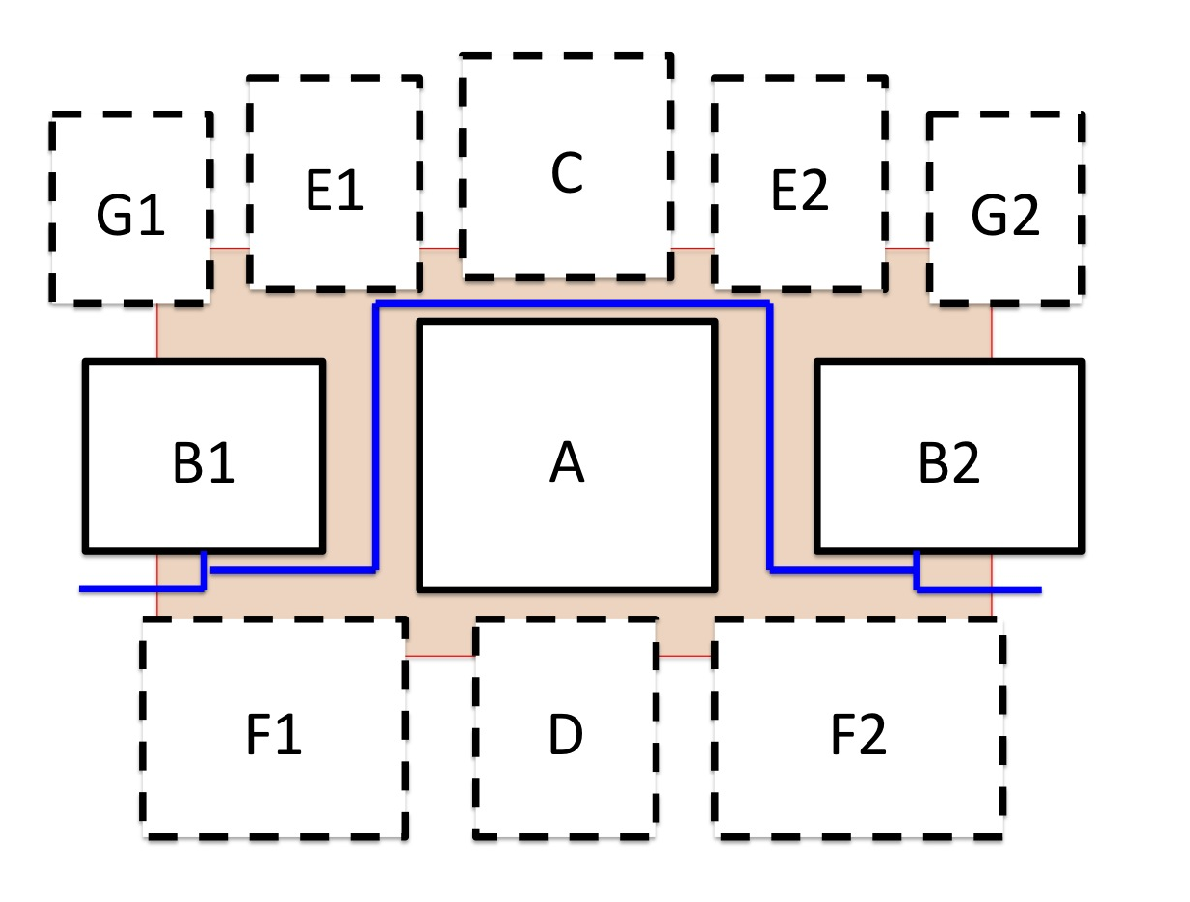
\includegraphics[width=4cm]{Fig/RoutingPreserv_a.eps}
    \caption{Reference template layout}
    \label{fig:RoutingPreserv_A}
    \end{subfigure}
    \begin{subfigure}[t]{4cm}
    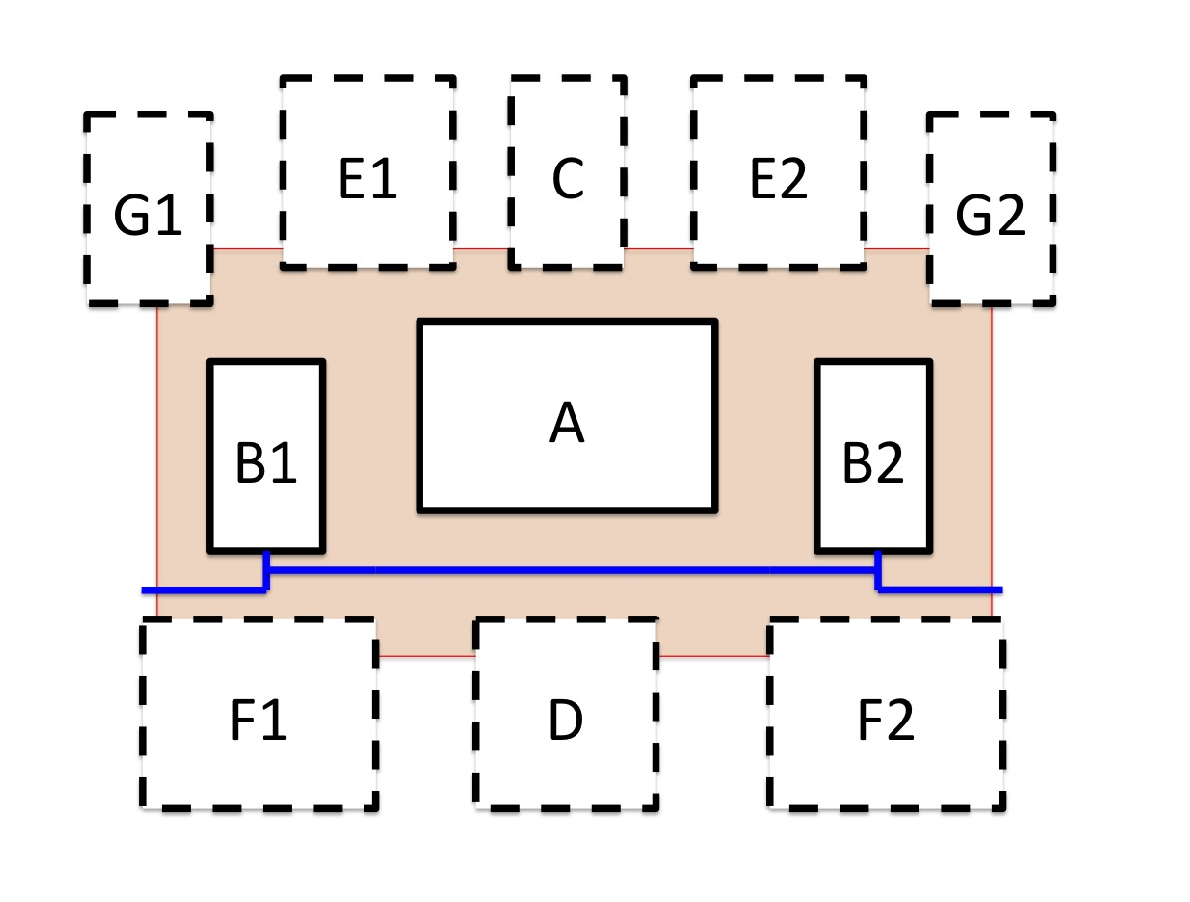
\includegraphics[width=4cm]{Fig/RoutingPreserv_b.eps}
    \caption{Non-preserved automatic routing}
    \label{fig:RoutingPreserv_B}
    \end{subfigure}
    %}
    \begin{subfigure}[t]{4cm}
    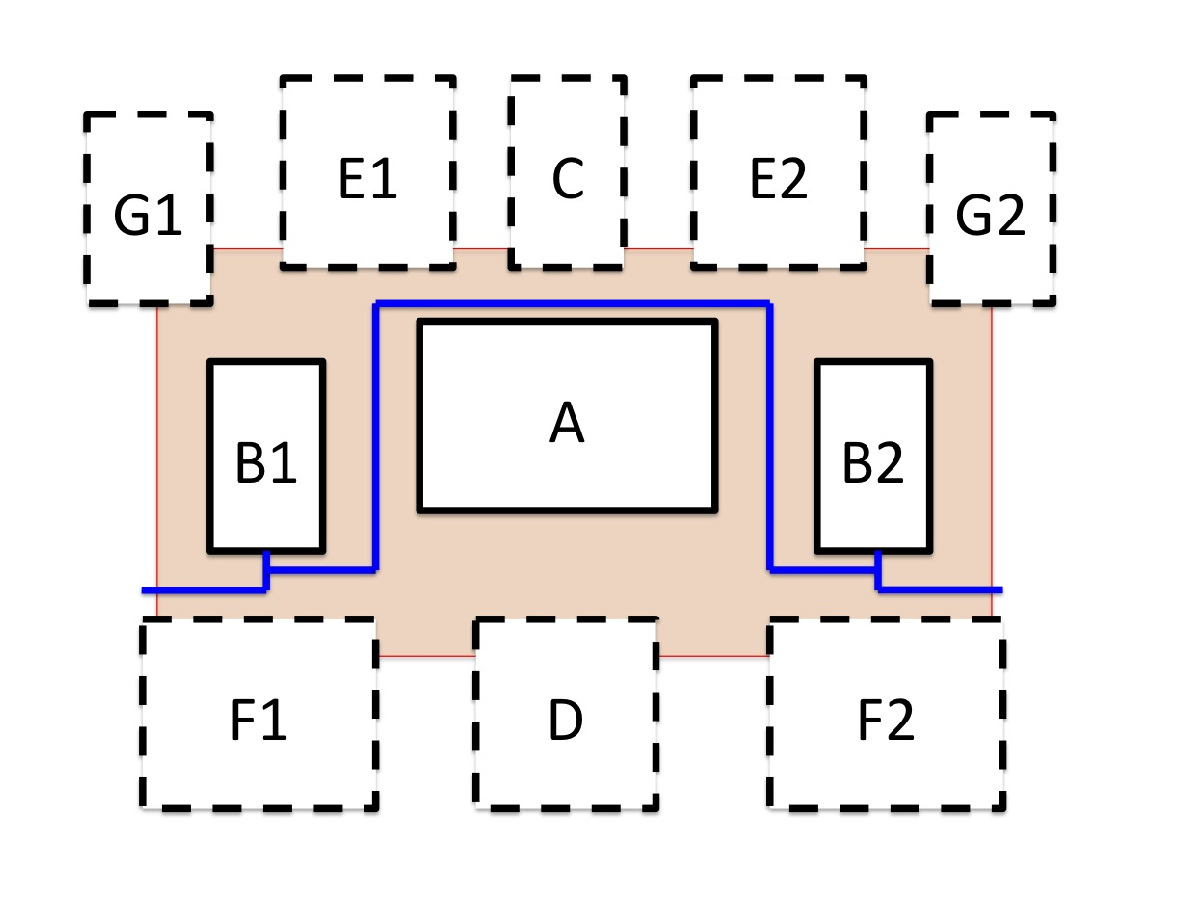
\includegraphics[width=4cm]{Fig/RoutingPreserv_c.eps}
    \caption{Preserved routing}
    \label{fig:RoutingPreserv_C}
    \end{subfigure}
    %}
    
    %\subfigure[Timing and simulation results]{
    %\label{fig:RoutingPreserv_d}
    %\epsfig{file=Fig/Prototyping_d.eps,width=4cm}
    %}
    \caption{Analog layout generation with different configuration. (a) Reference layout with complete placement and routing. (b) non-preserved automatic routing considering usual constraints only. (c) layout generation considering preserved routing characteristics. (d) simulation results in umc65nm technology.}
    \label{fig:RoutingPreserv}
  \end{figure}
% !TEX root = Thesis.tex

\chapter{Preliminaries}\label{chap:prelim}

  \newtheorem{defi}{Definition}

  In this section, we first raise the motivation to utilize triangulation for analog layout migration in Chapter~\ref{sec:WhyCDT}, and later review the planar straight-line graph (PSLG) and the corresponding constrained Delaunay triangulation (CDT)~\cite{CDT} in Chapter~\ref{sec:Review}. In the end, we define the analog layout prototyping problem in Chapter~\ref{sec:problem}.

  \section{Routing Preservation with Planar Triangulation}\label{sec:WhyCDT}

    To facilitate the routing preservation in the existing layout, the relationship between routing wires and placement blocks is crucial. The triangulation of layout plane is used to take down the correlation. Fig.~\ref{fig:WhyCDT} depicts that the updated triangular edges can retain the routing behavior among blocks after shrinking and stretching. Therefore, planar triangulation is applied to our analog layout migration mechanism.

    \begin{figure}[ht]
      \begin{center}
        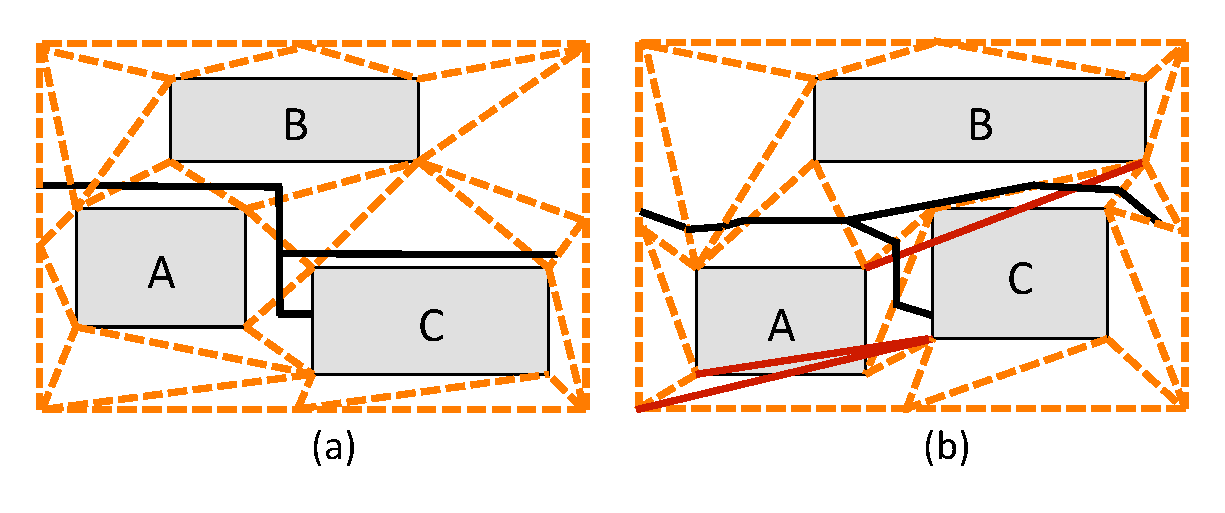
\includegraphics[width=\textwidth]{Fig/WhyCDT.eps}
        \caption{Illustration of triangulation to take down the correlation between placement and routing. (a). The existing layout with triangles at routing channel. (b) The migrated layout with updated triangular edges and recovering routing paths.}
        \label{fig:WhyCDT}
      \end{center}
    \end{figure}

  \section{Review of PSLG and CDT}\label{sec:Review}

    In order to describe the analog layout design as a planar straight-line graph (PSLG), we briefly define PSLG as follows:

    \begin{defi}\label{defi:PSLG}
      A PSLG is a graph $G(V,E)$, which can be embedded in the plane without any crossing. Every edge $E$ in $G$ is a straight segment, where $V$ implies all the vertices in $G$ and $E$ implies all the edges connected to $V$. 
    \end{defi}

    By definition~\ref{defi:PSLG}, we can use PSLG to describe the placement of the analog layout with several rectangles and polygons. Furthermore, polygons decomposition is facilitated by decomposing into simpler components such as triangles. The triangulation can be generalized to a PSLG, where the entire plane is decomposed into triangles. The triangulation is defined in the following definition.

    \begin{defi}\label{defi:Triangulation}
      Triangulation is a process to produce an updated PSLG $G'(V'E')$ out of a given PSLG $G(V,E)$, such that each edge $e' \in E'$ is exactly a triangular edge.
    \end{defi}

    The complexity of triangulation is $O(n\log n)$, which is well explained in \cite{CDT}. We further look for a quality triangulation instead of triangles with arbitrary shapes. Therefore, the Delaunay Triangulation generates a set of points satisfying the empty circumcircle property, which maximizes the minimum angles. Therefore, CDT can minimize the number of triangles with small angles among placement blocks in the layout. In other words, CDT reduces the total number of triangular angles the routing wires should intersect. Additionally, in a practical analog layout problem, not all polygons and rectangles are supposed to be decomposed into triangles, such as obstacles and devices. The generalized Delaunay triangulation, which is also called constrained Delaunay triangulation (CDT), fit better for our requirement. 

    According to above definitions, it is possible to decompose the analog layout with obstacles and routing channels into convex holes and triangles, where the quality triangles are capable of preserving the across wires. 

  \section{Problem Description}\label{sec:problem}

    In this work, we aim at an analog layout migration problem by layout prototyping. 
    The problem can be described as follows:

    \newcommand{\tabincell}[2]{\begin{tabular}{@{}#1@{}}#2\end{tabular}}
    \newsavebox{\tablebox}


    \begin{itemize}
    \item 
    {\bf Analog Layout Migration Problem} 
    Given a source layout $L$ with technology information $T$, the main purpose is to produce a new $L'$ on target technology $T'$. The original layout $L$ comprises a set of placement modules $M$ and nets $N$, which consisting of at least one wire segment. Our objective is to provide multiple layout solutions. These layout solutions make more opportunities for designers to generate the appropriate layout much faster.
    \end{itemize}

    
% !TEX root = Thesis.tex
\chapter{Layout Migration Flow}\label{sec:migration}

  In this section, we introduce the overall flow of the proposed layout migration methodology.
  Generally, analog design follows hierarchical design concept that produces structural design. 
  Hence, to extend the idea, we also consider the multilevel analog design in our prototyping framework.Fig.~\ref{fig:Flow} shows the overall flow diagram.
  The flow is mainly separated into 3 stages: 1) the layout extraction and preservation stage, 2) the layout prototyping stage and 3) the wire segment refinement. 
  
  
  \begin{figure}[ht]
  \centering
  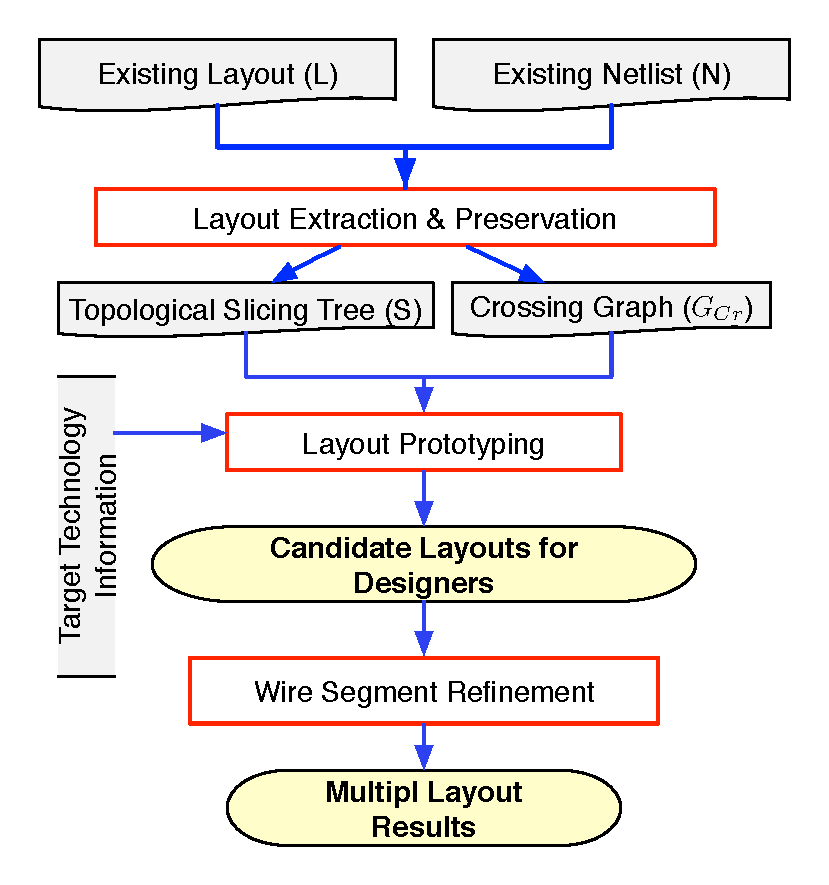
\includegraphics[width=0.5\textwidth]{Fig/Flow.eps}
  \caption{Overall flow of the proposed layout migration scheme.} 
  \label{fig:Flow}
  \end{figure}

  \begin{table}
    \begin{center}
    \caption{Comparison on Analog Layout Migration Approaches}\label{table:MigrateComp}
    \scriptsize
    %\begin{tabular}{|m{2cm}|m{2cm}|m{2cm}|m{2cm}|m{2cm}|}
    \begin{tabular}{|c|c|c|c|c|}
      \hline
      & \cite{msc-bhattacharya-tcad06} & \cite{ALP_YPWeng_iccad2011} & \cite{Chin_DMR_ICCAD2013} & Our Approach \\
      \hline
      Layout Constraints & Preserved & Preserved & Preserved & Preserved \\
      \hline
      Placement topology  & Keep origin & Multi-prototypes & Already given & Multi-prototypes \\
      \hline  
      Routing behavior  & Partially preserved &  Manually completed &  Preserved routing & Preserved routing \\
      \hline
      \#Migrated Layout &  1 &  Multi-Solutions & Multi-Solutions & Wires refined Multi-Solutions \\
      \hline
      Sign-off Time &   slow &  slow &  fast &  fast \\
      \hline
    \end{tabular}
    \end{center}
  \end{table}

  In comparison with current migration mechanisms, Table~\ref{table:MigrateComp} shows the different criterion to examine the disparity. There are 3 current migration styles, \cite{msc-bhattacharya-tcad06}, \cite{ALP_YPWeng_iccad2011} and \cite{Chin_DMR_ICCAD2013}, mentioned in Table~\ref{table:MigrateComp}. For analog layout constraints, each approach is able to preserve specific constraints such as symmetry constraints and matching constraints. For placement topology, \cite{msc-bhattacharya-tcad06} aims to keep the exactly same topology as the existing layout, \cite{ALP_YPWeng_iccad2011} successfully produces multiple placement candidates and the placement in \cite{Chin_DMR_ICCAD2013} is already given. For routing behavior, \cite{msc-bhattacharya-tcad06} only preserves the wires that belong to the symmetric devices or clusters which are symmetric on the original layout, \cite{ALP_YPWeng_iccad2011} manually completes the routing section and \cite{Chin_DMR_ICCAD2013} quickly produces routing prototype with routing preservation. 

  Therefore, \cite{msc-bhattacharya-tcad06} generates single layout each time and \cite{ALP_YPWeng_iccad2011} can generate multiple layout solutions. \cite{Chin_DMR_ICCAD2013} produces multiple solutions from multiple placement results. To consider the Time-to-sign-off for overall flow, \cite{msc-bhattacharya-tcad06} and \cite{ALP_YPWeng_iccad2011} are slower due to the routing generation and \cite{Chin_DMR_ICCAD2013} facilitates the routing generation. In comparison, our approach consolidates the advantages from \cite{ALP_YPWeng_iccad2011} for more opportunity and \cite{Chin_DMR_ICCAD2013} for fast prototyping. Additionally, our approach refines the wires for better performance. In other words, we firstly generate multiple placement candidates and utilize them with preserved routing behaviors to fast generate multiple layout results. 


% !TEX root = Thesis.tex

\chapter{Layout Extraction and Preservation}\label{chap:LayoutExtPre}

  In this chapter, we emphasis on how to decompose the analog layout in placement and routing. We first divide the layout with blocks and wire segments, and later extract them respectively. The overall extraction flow is illustrated as Fig.~\ref{fig:ExtractFlow}. 

  \begin{figure}[t]
    \centering
    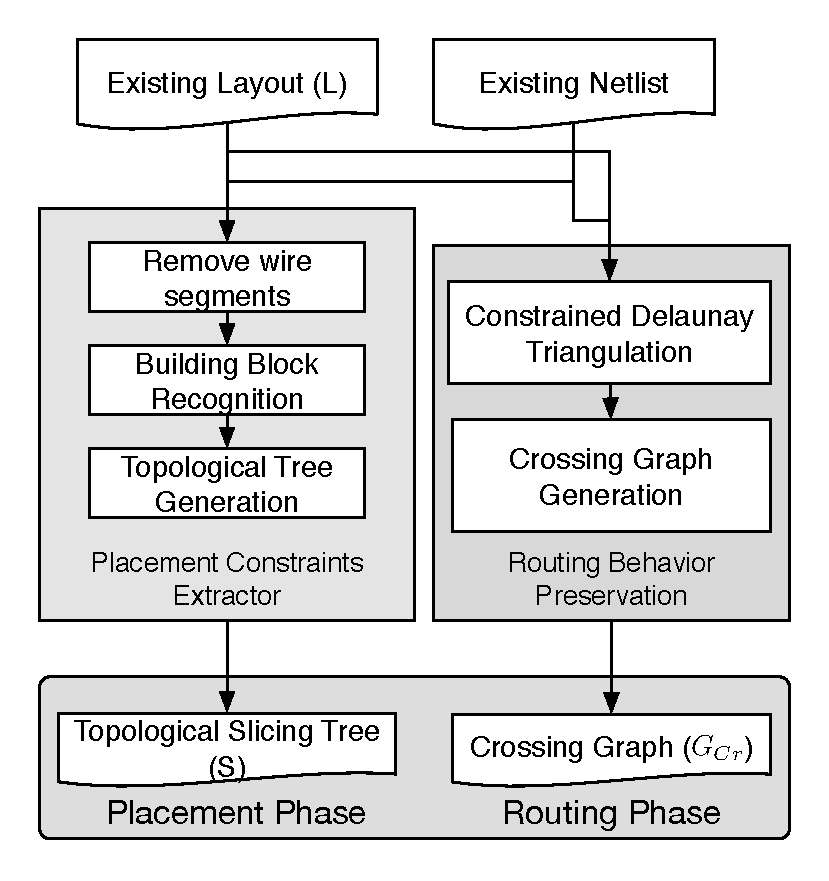
\includegraphics[height=7cm]{Fig/ExtractFlow.eps}
    \caption{The extraction separates layout into placement phase as topological slicing tree and as routing phase crossing graph.}
    \label{fig:ExtractFlow}
  \end{figure}


  \section{Placement Constraints Extraction}\label{sec:PlExtract}

    \begin{figure}[t]
      \begin{center}
      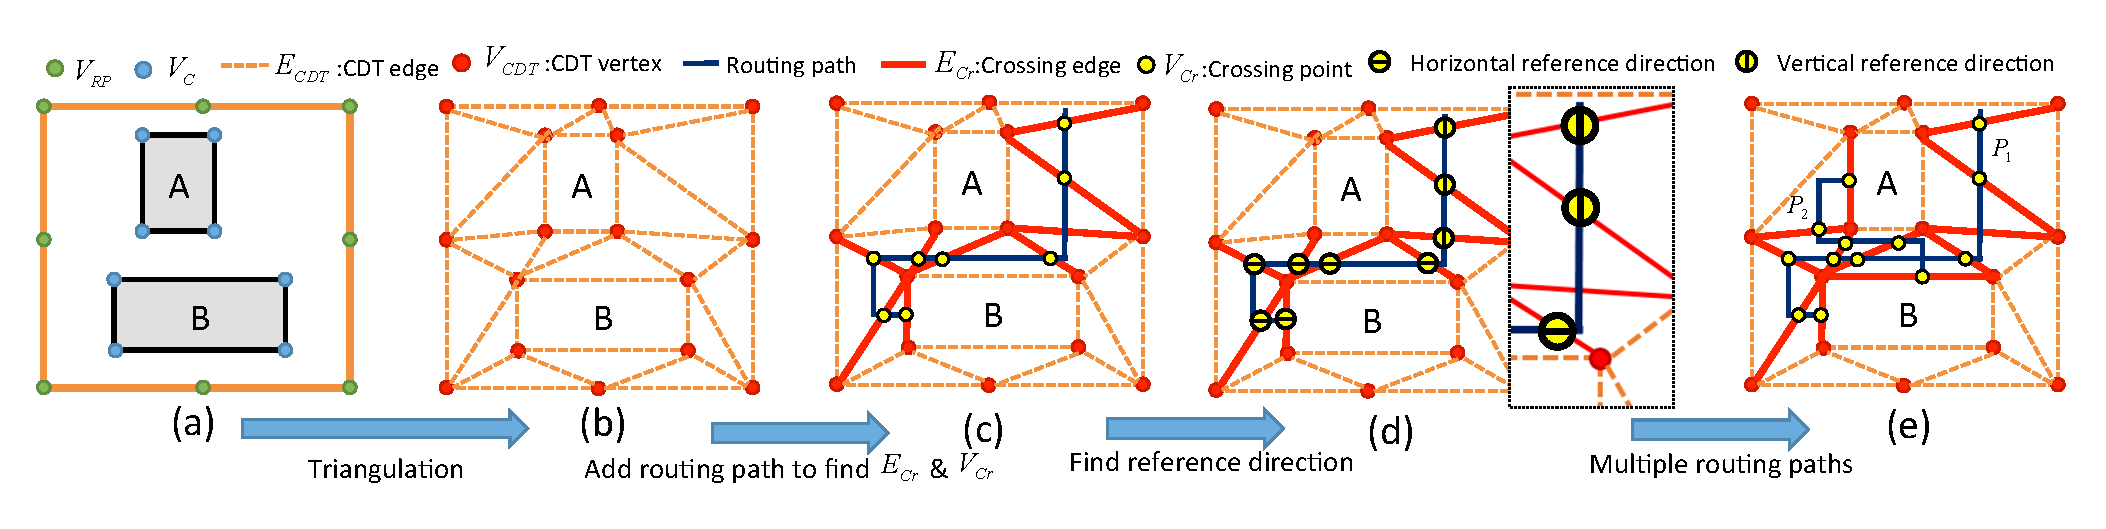
\includegraphics[width=\textwidth]{Fig/CGC.eps}
      \caption{Illustration of routing preservation by CDT. 
        (a) The given design.
        (b) Resultant CDT graph $G_{CDT}$.
        (c) CDT edges crossing with routing path are colored by red.
        (d) Crossing points of the two paths in routing plane.
        (e) Routing behavior is stored by CDT graph and the crossing points.}
      \label{fig:CGC}
      \end{center}
    \end{figure}

    %In the beginning of placement constraints extraction, we first remove the wire segments from the existing layout then implement extraction. 
    The major flow of placement constraints extraction \cite{ALP_YPWeng_iccad2011} is reviewed as follows:
    \subsection{Building Block Recognition}
      In order to reduce mismatch while generating layout, the principles of symmetrical and matching constraints should be considered as building blocks. 
      Besides, Building blocks under the same matching constraints are identified by the existing netlist. Via pattern matching technique \cite{Massier_TCAD08} the preferable matching building blocks are generated.

    \subsection{Topological Slicing Tree Generation}
      Later, these fundamental build blocks construct the topological slicing tree. In general, the placement can be decomposed by horizontal and vertical cuts. However, since some of the devices are recognized as build blocks, the traditional slicing tree tends to occur mismatches. Instead, cells under the same building block are placed together as a super-module in representation. After vertical and horizontal  partitioning, a topological slicing tree (S) with n symmetry groups, m matching groups which outside any symmetry group, and l non-symmetry cells in layout are generated at the same hierarchy. Other than \cite{ALP_YPWeng_iccad2011} which flattens the layout into the unit hierarchy for slicing tree generation, we preserved the hierarchy of the layout with respect to the hierarchical structure from the existing netlist. Such hierarchy is essential for multi-level layout reconstruction. 




  \section{Routing Preservation via Crossing Graph Construction}\label{subsec:CGC}


    \newcommand{\CCG}{\ensuremath{\mbox{\sc ConstCrossGraph}}}
    \renewcommand{\algorithmicrequire}{\textbf{Input:}}
    \renewcommand{\algorithmicensure}{\textbf{Output:}}
    \begin{algorithm}[hbt]  
      \caption{$\CCG(P,B,V_{RP})$}\label{alg:CCG}                       
      \begin{scriptsize}
        \begin{algorithmic}[1]
          \REQUIRE 
            \begin{tabular}{l}
              $P$: The routing paths of layout\\
              $B$: The placement blocks \\
              $V_{RP}$: Corners of layout and the middle-points of each plane boundary\\ 
            \end{tabular}
          \ENSURE 
            \begin{tabular}{l}
              $T$: The triangles after CDT\\
              $E_{CDT}$: The edges set of $G_{CDT}$\\
              $V_{Cr}$: The set of crossing points between routing paths and $E_{CDT}$\\
              $E_{Cr}$: The set of crossing edge\\
              $G_{Cr}$: The crossing graph
            \end{tabular}
          \FOR {$i = 1 \to |B|$}
            \STATE $V_C \gets v^{TR},v^{TL},v^{BR},v^{BL} $ \COMMENT{collect four corners into $V_C$}
          \ENDFOR
          \STATE $V_{CDT}\gets V_C, V_{RP}$  \label{line:VCDT}
          \STATE $G_{CDT}(V_{CDT},E_{CDT},B,T) \gets CDT(V_{CDT},B)$  \COMMENT{constrained Delaunay triangulation} \label{line:GCDT}
          \FOR {$i = 1 \to |P|$} \label{line:StartCross}
            \STATE $E_{Cr}(p_i) \gets CheckCrossEdge(p_i,E_{CDT})$
            \FOR {$j = 1 \to |E_{Cr}(p_i)|$}
              \STATE $v(x,y) \gets FindCross({E_{Cr}(p_i)}_j)$
              \STATE $q_1,q_2 \gets FindAdjacent({E_{Cr}(p_i)}_j,V_{CDT})$
              \STATE $V_{Cr}(p_i) \gets v,q_1,q_2$
            \ENDFOR
            \STATE $E_{Cr} \gets E_{Cr}(p_i)$
            \STATE $V_{Cr} \gets V_{Cr}(p_i)$
          \ENDFOR \label{line:EndCross}
          \RETURN $G_{Cr}(V_{CDT}\cup V_{Cr}, E_{CDT} \cup E_{Cr},B,T)$  
        \end{algorithmic}
      \end{scriptsize} 
    \end{algorithm}

    This Section introduces a new representation to preserve the routing correlation with placement. As Fig.~\ref{fig:WhyCDT}.(a) illustrated, the routing channel can be decomposed into multiple triangles via CDT. Thus, the wire goes across one or more triangles on their edges. The representation which aims to record the "crossing" behavior among wires and triangular edges is denoted by a crossing graph. The crossing graph construction is demonstrated in the following paragraph. 


    Fig.~\ref{fig:CGC} illustrates a routing preservation procedure and Algorithm~\ref{alg:CCG} {\it ConstCrossingGraph} represents it as a pseudocode. Given a layout plane $L$ with a set of placement blocks $B \in L$, where $B = \{b_i|1 \leq i \leq |B|\}$. As the layout without routing path shown in Fig.~\ref{fig:CGC}.(a), the set of corner points of blocks in $B$ are denoted by $V_C$ where $V_C = \{(x_i,y_i)|1 \leq i \leq 4|B|\}$, and the points on the periphery of routing plane (i.e. corners of the routing plane and the middle-points of each routing plane boundary) are denoted by $V_{PR}$. We define the vertex set of the layout extraction CDT to be $V_{CDT} = V_C \cup V_{RP}$ in line~\ref{line:VCDT}. Regions that forbid CDT edge are called {\it blocks} in CDT formulations. In our case, they are the areas inside blocks.


    As shown in line~\ref{line:GCDT}, the CDT graph $G_{CDT}$ generated from vertex set $V_{CDT}$ and block set $B$ can be represented as $G_{CDT} = \{V_{CDT},E_{CDT},B,T\}$, where the edge set $E_{CDT} = \{(v_i,v_j)|v_i,v_j\in V_{CDT}\}$ splits the plane into a set of non-overlapping triangles $T$ and the rectangular blocks $B$. According to Fig.~\ref{fig:CGC}.(b), the layout with 2 blocks are transferred into a $G_{CDT}$ after triangulation, where $|B|$=2 (block A and B), $|V_{CDT}|=16$, $|E_{CDT}|=34$ and $|T|=18$.


    After $G_{CDT}$ is established, one routing path is recovered back to demonstrate the routing preservation. As displayed in Fig.~\ref{fig:CGC}.(c), one $e_{CDT}$ intersects with the routing path is denoted by a crossing edge $e_{Cr}$ and the intersected point is denoted by a crossing point $v_{Cr}$. The detailed definition is as follows:

     
    \begin{defi}\label{defi:CrossingPoint}
      Given a routing path $p$, and CDT edge set $E_{CDT}= \{e_{CDTi}| 1 \leq i\leq|E_{CDT}|\}$, if there exists a point $v(x,y)$ which is both on $p$ and $e_{CDTi}$, $e_{CDTi}$ is a crossing edge $e_{Cr}$ and $v(x,y)$ is a crossing point $v_{Cr}$.
    \end{defi}

    From line~\ref{line:StartCross} to line~\ref{line:EndCross} in Algorithm~\ref{alg:CCG}, the procedure traverses the set crossing edges $E_{Cr}$ and crossing points $V_{Cr}$ is delivered. As Fig.~\ref{fig:CGC} displayed, an orange dotted line which originally denotes $e_{CDT}$ changes into solid red line as a crossing edge $e_{Cr}$, and the yellow point represents the intersection between the routing path, and such intersected point denotes a crossing point $v_{Cr}$. In addition, each $v \in V_{Cr}$ belongs to a routing path along with a crossing direction (horizontal/vertical, H/V), as illustrated in Fig.~\ref{fig:CGC}.(d). The directions are treated as {\it reference directions} which will be used later in the routing reconstruction stage, described in Section~\ref{chap:prototyping}. 



    For multiple nets design, a single edge might be crossed with two or more routing paths. As illustrated in Fig.~\ref{fig:CGC}(e), the two routing paths, $p_1$ and $p_2$, both pass through space between block A and B with $p_2$ closer to block A. In order to preserve the behavior of multiple nets routing, we define the {\it crossing graph} $G_{Cr}$ of layout $L$ as follows:
    \vspace{0.2cm}
    \begin{defi}\label{defi:CrossGraph}
      Let $G_{CDT}(V_{CDT},E_{CDT},B,T)$ denotes the CDT graph of $L$. $V_{Cr}$ denotes the set of crossing point and $E_{Cr}$ denotes the set of crossing edges. Then graph $G_{Cr} = \{V_{CDT} \cup V_{Cr},E_{CDT} \cup E_{Cr},B,T\}$ is a crossing graph of layout $L$. 
    \end{defi}
    \vspace{0.2cm}
    In the end, the crossing graph stores not only the individual routing topology, but also the relative order of paths within each routing channel.


  \section{Hierarchical Layout Extraction and Preservation}\label{sec:HLE}

    \begin{figure}[t]
      \begin{center}
      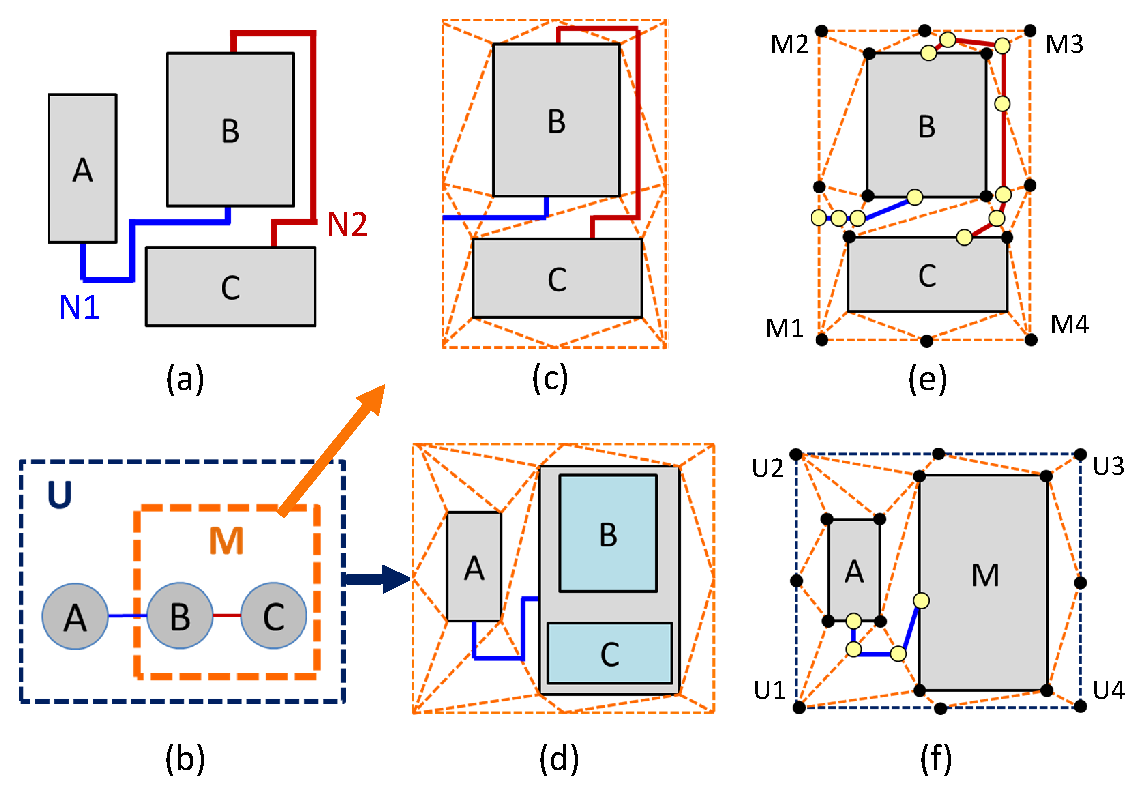
\includegraphics[width=8.5cm]{Fig/HIER.eps}
      \caption{
         (a) A layout with 3 placement blocks and two routing paths. 
         (b) Hierarchical Structure of (a).
         (c) CDT graph of cluster M (bottom level cluster).
         (d) CDT graph of cluster U (upper level cluster).
         (e) Corresponding crossing graph of (c).
         (f) Corresponding crossing graph of (d), cluster M is regarded as a placement block here.
        }
      \label{fig:HIER}
      \end{center}
    \end{figure}

    In order to reduce mismatches, the symmetry and proximity constraints need to be considered for both placement and routing. 
    For the given source layout, modules/devices are grouped as clusters according to the symmetry and proximity constraints, 
    where the constraints can be either given by designers or extracted from the source layout as in Section~\ref{sec:PlExtract}.

    For each cluster, the routing behavior and correlation with placement blocks are analyzed based on the CDT of that cluster to build a corresponding crossing graph. 
    Crossing graphs of clusters are constructed bottom-up along the hierarchical structure. 
    Bottom-level clusters are regarded as placement blocks in upper-level clusters. 
    Consequently, a series of crossing graphs is generated which contain the routing behavior hierarchically.

    Fig.~\ref{fig:HIER} illustrates this multilevel crossing graph generation.
    Fig.~\ref{fig:HIER}(a) shows a simple layout with three blocks and two nets.
    Assume block B and C are grouped into cluster M, and M and A are grouped into U as shown in Fig.~\ref{fig:HIER}(b).
    According to the hierarchy, two crossing graphs are constructed with respect to cluster M and U, and
    each routing path is divided into 1) intra-cluster connections and 2) inter-cluster connections. 
    As illustrated in Fig.~\ref{fig:HIER}(c)(d), path N1 is segmented into inside parts and outside parts of M. 
    Therefore, the crossing points of N1 appear in both two crossing graphs. 
    On the other hand, since N2 contains only intra cluster connection in M, the corresponding crossing points are all inside a single graph. 

    


%%!TEX root = Thesis.tex

\chapter{Conclusions and Future Works}\label{chap:CFW}

  \section{Conclusions}\label{sec:Conclusion}

    This dissertation presents a methodology of analog circuit optimization, an unification of analog design constraints and a framework of analog layout migration. 

    \begin{itemize}
      \item In analog circuit design procedure, front-end synthesis and physical layout generation play distinctive roles to optimize the circuit performance. On circuit synthesis phase, in order to figure out the limitation of the manufacturing technology for circuit sizing, we develop a performance exploration methodology via parallel genetic algorithm. First of all, a potential performance space for optimized solution is explored based on parallel genetic algorithm. Later, such performance space is transferred into device-variable domain for a probabilistic simulation. A RFDA and an Op-Amp circuit are practiced to demonstrate the effectiveness. Our proposed approach efficiently reduces the runtime and obtains qualified performance. 
      \item Between the gap of netlist and layout design, the constraints according to circuit design are critical to layout generation. The LDEs from advanced manufacturing technology of integrated circuit are also decisive to layout performance. We propose a unified constraint group to integrate the technology and design constraints as guidelines for layout generation. The proposed HCDR reconfigures the analog routing order according to the unified constraint group. In addition, different combinations of constraint group generate routing by HCDR automatically. Our experiment results show that analog layouts with HCDR obtain better performance than non-constrained router especially on signal integrity perspective. 
      \item Template-based layout generation is widely-discussed in state-of-the-art of analog circuit automation. Given an existing analog layout design, we perform a rapid design migration framework to generate layout prototypes on the targeting technology. We firstly represent the layout as a slicing tree and use crossing graph for feature preservation, and then a prototyping flow is implemented to generate multiple layout candidates efficiently. Additionally, a wire segment refinement enhances the routing characteristics for better performance. The proposed approach is validated on a variable-gained amplifier, a folded-cascode Op-Amp and a low drop-out regulator. Experimental results show that our approach preserves analog layout and migrates efficiently. The migrated layout reduces the effort of manual routing with at least on 75\% wirelength and 80\% on wire segments. As a result, this work speeds up at least 5 times over manual layout generation. 
    \end{itemize}

  \section{Future Works}\label{sec:FW}


    As the hardship of analog design expands in the advanced technology, the demand of LDE before layout generation increases. To enhance the efficiency to explore the optimized performance is quite important. In Chapter~\ref{chap:PAGE}, the evolutionary methodology should take LDE into consideration. Moreover, the aging model of device can also be part of device fitting. In the performance exploration stage, since the initial solution of genetic algorithm dominates the evolved solution, the optimized circuit sizing vary each time. It is possible to use the design variables' values from the existing circuit as an inital solution. Additionally, the power dissipation and the area should be minimized other than satisfying the performance specification. 

    In Chapter~\ref{chap:CUCLM}, even though the unified constraint groups can develop the analog routing for signal integrity, the idea can be combined with the migration framework in Chapter~\ref{chap:RLPADM}. According to Table~\ref{table:HCDRResult}, the number of VIAs and DRC errors still have room to develop, it is possible to describe the VIA issue during constraint generation. For design rule checking, the layout migration approach also needs improvement in detail routing to fix the illegal layers. Nonetheless, the future work will mainly focus on the extension of the configurable analog constraints like electromagnetic effect, and on the symbolic routing with such configurable analog constraints for better performance.

    In the end, the preserved representation of analog layout is divided into placement and routing phase in Chapter~\ref{chap:RLPADM}. The CDT as our layout preservation strategy have not fulfilled itself. We will dedicate to develop a unified representation for layout preservation to simplify analog layout migration. Additionally, in order to automatically migrate analog layout, the completeness of prototyping layout still has space to develop. We plan to automatically generate the detailed components of each prototype so that the efficiency of our migration will be boosted. 
%\input{Thesis_Chapter6.tex}



\backmatter
% !TEX root = Thesis.tex
% this file is encoded in utf-8
% v2.0 (Apr. 5, 2009)


%%%
\newpage
%\phantomsection % for hyperref to register this
%\addcontentsline{toc}{chapter}{\nameRef}
%\renewcommand{\bibname}{\protect\makebox[5cm][s]{\nameRef}}
%%  \makebox{} is fragile; need protect
\bibliographystyle{IEEEtran}  % �ϥ� IEEE Trans ���Z�榡
\bibliography{IEEEabrv,reference,reference_PAGE,reference_HCDR}


%%%
%\input{my_appendix.tex}

%%%
\newpage
\chapter*{\protect\makebox[\textwidth][c]{\nameVita}} % \makebox{} is fragile; need protect

\phantomsection % for hyperref to register this
\addcontentsline{toc}{chapter}{\nameVita}
%!TEX root = Thesis.tex

{\bf Po-Cheng Pan} received the B.S. degree in electronics engineering from National Chiao Tung University, Hsinchu, Taiwan, in 2007. 

From 2007, he we working his M.Sc. degree in electronics engineering. From 2009, he is currently pursuing the Ph.D. degree from the Institute of Electronics. He was a visiting scholar in Technical University of Munich in 2014 through DAAD program. His research interests includes analog circuit optimization, and analog circuit layout automaiton and migration. 

{\bf International Journal Papers}
\begin{enumerate}
  \item P.-C. Pan, C.-Y. Chin, H.-M. Chen, T.-C. Chen, C.-C. Lee and J.-C. Lin, ``A Fast Prototyping Framework for Analog Layout Migration with Planar Preservation,'' in \emph{IEEE Transactions on Computer-Aided Design of Integrated Circuits and Systems}, vol.pp, no.99, pp.1---1. 
\end{enumerate}
{\bf International Conference Papers}
\begin{enumerate}
  \item C.-Y. Chin, P.-C. Pan, H.-M. Cheng, T.-C. Chen, and J.-C. Lin, ``Efficient analog layout prototyping by layout reuse with routing preservation,'' in \emph{International Conference on Computer-Aided Design}, Nov. 2013, pp.40---47.
  \item P.-C. Pan, H.-M. Chen and C.-C. Lin, ``PAGE: Parallel agile genetic exploration towards utmost performance for analog circuit design,'' in \emph{Design, Automation and Testing in Europe Conference \& Exhibition}, Mar. 2013, pp.1849---1854.
  \item P.-C. Pan, H.-M. Chen, Y.-K. Cheng, J.~Liu, and W.-Y. Hu, ``Configurable analog routing methodology via technology and design constraint unification,'' in \emph{International Conference on Computer-Aided Design}, Nov. 2012, pp.620---626.
  \item Y.-P. Weng, H.-M. Chen, T.-C. Chen, P.-C. Pan, C.-H. Chen, and W.-Z. Chen, ``Fast analog layout prototyping for nanometer design migration,'' in \emph{International Conference on Computer-Aided Design}, Nov. 2011, pp. 517 -- 522.
  \item K.-H. Meng, P.-C. Pan, and H.-M. Chen, ``Integrated hierarchical synthesis of analog/rf circuits with accurate performance mapping,'' in \emph{International Symposium on Quality Electronic Design}, Mar. 2011, pp.1---8. 
  \item B.-Z. Chen, H.-M. Chen, L.-D. Huang and P.-C. Pan, ``A stochastic-based efficient critical area extractor on OpenAccess platform,'' in \emph{ACM Great Lake symposium on VLSI}, May 2009, pp.197---222.

\end{enumerate}



\end{document}
